\documentclass[a4paper,10pt]{IEEEtran}
\usepackage[utf8]{inputenc}
\usepackage{graphicx}

%opening
\title{Large Scale Web Page Optimization of Virtual Labs}
\author{Utkarsh Rastogi, Prateek Pandey, Maddala Saraswati Soumya, Jatin Agarwal and Venkatesh Chopella}

\begin{document}

\maketitle

\begin{abstract}
We propose web page optimization as necessary step in web application development. In context of virtual labs were several online
experiments were designed by domain experts from various disciplines thousands of web pages were developed. But domain expert 
would not know best practices for web development, therefore end user suffer from  performance issues. Performance of an web
application largely depends upon the content of the web page because rendering takes place on client side. And client machine may
have limited resources at his side. Therefore web page optimization seems an necessary step to improve user experience. In this
paper we will describe approach we have used to analyze and optimize web pages for huge website like virtual labs. 
\end{abstract}

\section{Introduction}
In today's world any interactive web application is judged based on user experience. Even though world is moving on
cloud web servers but rendering of page is done on the client side. So if the content of the web page was developed with out
considering best practices listed by web giants like yahoo and google than it renders very slowly. These days web pages 
contain many critical resources like css files, java script files, images etc. 

Virtual 

\section{Previous Work}
We use ylsow.js as our performance mesuring tool of a web page. Yslow.js analyses web pages and why they are slow based on Yahoo's
rules for high performance web sites. We use ylsow because it not only grades web pages based on a prefined ruleset but also offers
sugestions for improving web performance.
\section{Experimentation}
Our work is broadly divided into four major phases namely Data Collection, Data Visualization, Analysis of Data and
optimizing web pages based on analysis. During data collection phase we first collected all the urls of virtual labs hosted at IIIT Hyderabad.
Then we collected yslow reports for each web page using an automated script and phantomJS. After collecting all the reports we extracted scores
for each rule from reports and stored it in a csv file. During visualization phase all data is visualized using an automated script indicating
performance for each rule and also overall performance of web pages. Later we did analysis for optimizing web pages of virtual labs. 

\subsection{Url and Report Collection}
In this section we describe approaches used to collect all the urls of virtual-labs.ac.in and automated mechanism to generate reports for
thousands of web pages. We will also explain significance of automated report generation using Ylsow and phantomJS.
\subsection{CSV file generation}
In this section we explain our logic to extract relevant fields from Ylsow reports and accumulate all the scores of each url into a single CSV file to
simplify analysis to get better understanding of existing performance issues and to get insights on what need to be optimized.
\subsection{Score Visualization}
In this section we talk about automated visualizing tool from the data accumulated 

\section{Analysis}
In this section we analyze web page performance of virtual-las.ac.in in two different settings on data set containing 9000 web pages.
One when page speed module is installed on our system and other one without page speed. We also analyze web page performance of vlab.co.in  
on data containing 5000 web pages. Based on analysis we can provide suggestions on how to improve the performance. 
\subsection{Analysis of vlabs.co.in}
hello
\subsection{Analysis of virtual-labs.ac.in}
\begin{figure}[ht]
 \centering
$\includegraphics[scale=0.27]{images/Overall_Score_vlab.jpg}$
\caption{}
\label{fig1}
\end{figure}



\begin{figure}[ht]
 \centering
$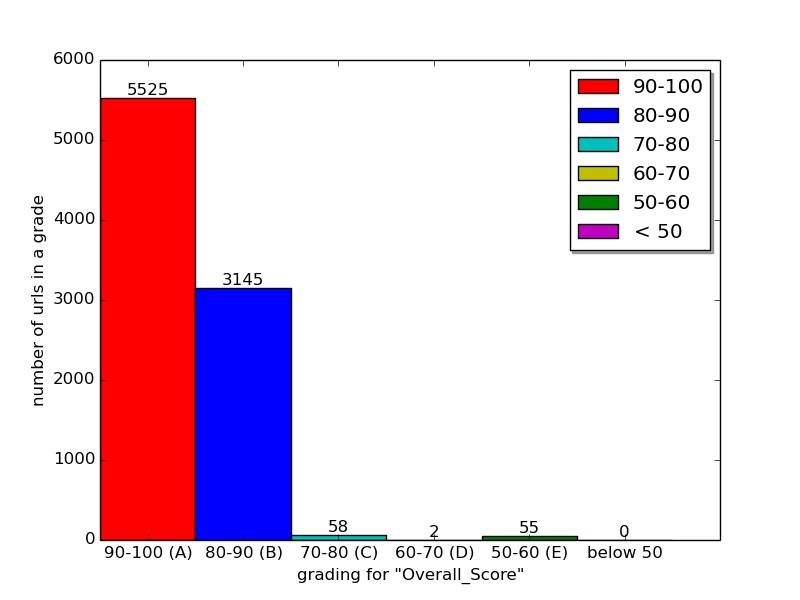
\includegraphics[scale=0.27]{images/Overall_Score_deploy.jpg}$
\caption{Overall Scores of 9000 urls using without pagespeed installation}
\label{fig1}
\end{figure}

\begin{figure}[ht]
 \centering
$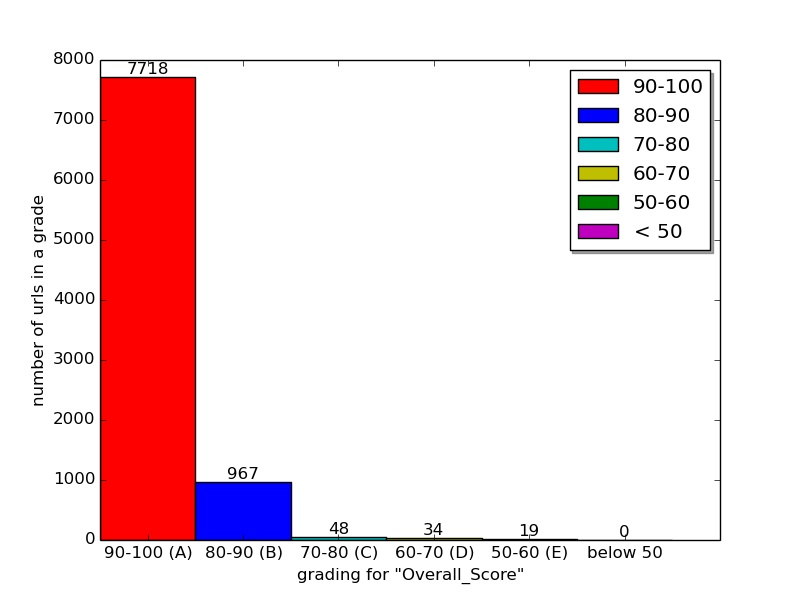
\includegraphics[scale=0.27]{images/Overall_Score_container.jpg}$
\caption{Overall Scores of 9000 urls using pagespeed installation}
\label{fig2}
\end{figure}

\section{Page Speed and Web page Optimization}
In this section we explain about significance of page speed in context of Virtual Labs project and its wide applicability. We also explain
in detail about page speed filters and their limitations. 

\section{Conclusion}


\end{document}
